% TrinCore_Paper.tex
\documentclass[11pt,a4paper]{article}

% ---------- Packages ----------
\usepackage[T1]{fontenc}
\usepackage[utf8]{inputenc}
\usepackage{times}
\usepackage{microtype}
\usepackage{geometry}
\geometry{margin=1in}
\usepackage{setspace}
\onehalfspacing
\usepackage{graphicx}
\usepackage{caption}
\usepackage{subcaption}
\usepackage{booktabs}
\usepackage{multirow}
\usepackage{array}
\usepackage{enumitem}
\usepackage{xcolor}
\usepackage{hyperref}
\hypersetup{
  colorlinks=true,
  linkcolor=blue!60!black,
  citecolor=blue!60!black,
  urlcolor=blue!60!black
}
\usepackage{siunitx}
\sisetup{detect-all}
\usepackage{listings}
\usepackage{amsmath,amssymb,amsthm}
\usepackage{mathtools}
\usepackage{tikz}
\usetikzlibrary{arrows.meta,positioning,shapes,calc}

% ---------- Listings (code) ----------
\lstdefinestyle{trincore}{
  basicstyle=\ttfamily\small,
  numbers=left,
  numbersep=6pt,
  frame=tb,
  framerule=0.4pt,
  columns=fullflexible,
  showstringspaces=false,
  breaklines=true,
  keywordstyle=\color{blue!60!black}\bfseries,
  commentstyle=\color{green!40!black}\itshape,
  stringstyle=\color{red!60!black},
  tabsize=2
}
\lstset{style=trincore,language=Python}

% ---------- Title ----------
\title{\vspace{-1em}\textbf{TrinCore: A Neuromorphic Ternary Computing Architecture}\\
\large Binary Compatibility, Event-Driven Processing, and a Quantum Bridge}
\author{
  Hemant \and TrinCore Team
}
\date{\today}

% ---------- Convenience macros ----------
\newcommand{\bitspertrit}{\ensuremath{\log_2 3 \approx 1.585}}
\newcommand{\project}{\textsc{TrinCore}}
\newcommand{\code}[1]{\texttt{#1}}
\newcommand{\trit}{\textit{trit}}
\newcommand{\trits}{\textit{trits}}
\newcommand{\figpath}{results}
\newcommand{\resbin}{results/binary_cpu}
\newcommand{\restern}{results/ternary_cpu}
\newcommand{\resneuro}{results/ternary_neuromorphic}
\newcommand{\resquant}{results/quantum}

% =========================================================
\begin{document}
\maketitle

\begin{abstract}
\project{} is a unified research platform that implements and compares three
CPU paradigms: a traditional binary CPU, a ternary CPU with higher data density,
and a neuromorphic (spiking) ternary CPU that executes workloads via event-driven
spike dynamics. The suite includes a master orchestrator, assembly-style
programming for custom workloads, a genetic algorithm module for learning logic
gates, and a quantum--ternary bridge with optional \emph{Qiskit} integration.
We report measured execution time, cycle counts, memory footprint, throughput,
accuracy, spike activity, and energy proxies, with artifacts and plots
automatically exported under \code{results/}. Our experiments show ternary logic
delivering \bitspertrit{} bits per symbol and neuromorphic execution achieving
meaningful event-driven efficiency with competitive accuracy, while remaining
binary-compatible and hardware-amenable (FPGA mapping). This paper documents
the architecture, methodology, datasets, and results; it is intended as a
research-grade reference and submission-ready record.
\end{abstract}

\tableofcontents
\listoffigures
\listoftables
\vspace{1em}

% =========================================================
\section{Introduction}
\label{sec:intro}
Binary computing has fueled decades of progress, but scaling pressure and
AI-centric workloads invite exploration of non-binary and event-driven
architectures. Ternary logic is a classical, well-studied alternative with
theoretical density benefits (\bitspertrit{}) and elegant arithmetic; neuromorphic
systems exploit sparse, event-driven computation inspired by spiking neurons.
\project{} unifies these lines of inquiry in a single codebase with
\emph{comparable simulators}, shared tooling, and reproducible outputs.

\paragraph{Contributions.}
\begin{itemize}[leftmargin=1.25em]
  \item A complete binary, ternary, and neuromorphic ternary CPU simulation
        suite with a master orchestrator and standardized metrics.
  \item A minimal assembly-style interface to define custom programs and
        evaluate instruction sets consistently across paradigms.
  \item A genetic evolution module that trains neural surrogates for logic
        gates and reports per-generation accuracy, enabling clear progress
        auditing (\S\ref{sec:nn}).
  \item Optional quantum components: entanglement demos and a conceptual
        quantum--ternary bridge (auto-detected if \emph{Qiskit} is installed).
  \item Polished reports with plots for execution time, cycles, memory,
        throughput, spikes, and energy proxies, emitted into
        \code{results/}.
\end{itemize}

% =========================================================
\section{Background and Related Work}
\label{sec:related}
\textbf{Ternary computing.} The Soviet \emph{Setun} machine and subsequent
balanced-ternary research motivate compact arithmetic and efficient carry
behavior. Modern studies revisit MVL (multi-valued logic) for memory density
and interconnect simplification.

\textbf{Neuromorphic computing.} IBM TrueNorth and Intel Loihi demonstrate
ultra-low-power, event-driven processing for AI kernels. Spiking neural models
offer temporal sparsity, fault tolerance, and locality.

\textbf{Quantum links.} Multi-valued logic connects naturally to higher-radix
qudits; while our project does not claim quantum advantage, it outlines a
\emph{bridge} for encoding ternary states into quantum circuits for pedagogy
and future research (\S\ref{sec:quantum}).

% =========================================================
\section{System Overview}
\label{sec:overview}
\project{} is organized as a modular Python codebase with three CPU backends,
shared utilities, and an orchestrator that executes end-to-end experiments
and writes a comprehensive comparison report.

\subsection{Repository Structure}
\begin{lstlisting}[language={},caption={Key directories in TrinCore},label={lst:layout}]
Applications/                 # Ternary CV and NLP demos
Cpu_components/               # ALU, registers, memory, ternary gates
FPGA_Simulator/               # Verilog emission, simple pipelines
Neuromorphic/                 # Spiking neurons, event-driven ALU, pipeline
NN/                           # Genetic evolution, models, training
Quantum/                      # Entanglement demo, quantum-spiking bridge
results/                      # All generated artifacts (.json, .png, .md)
\end{lstlisting}

\subsection{Master Orchestrator}
A single entry-point (\code{master\_main.py}) attempts to import and run
the full pipeline: binary $\rightarrow$ ternary $\rightarrow$ neuromorphic
$\rightarrow$ NN evolution $\rightarrow$ quantum (if available), and then
aggregates results into \code{results/comparison.md} plus a combined plot.

% =========================================================
\section{Architectures}
\label{sec:architectures}

\subsection{Binary CPU}
Our baseline binary CPU supports minimal bitwise operations and a small
assembly set (\code{LOADI}, \code{AND}, \code{OR}, \code{XOR}, \code{NOT},
\code{HALT}). It serves as a reference for timing, cycle counts, accuracy,
and memory footprint.

\subsection{Ternary CPU}
The ternary CPU generalizes arithmetic to mod~3 with \code{ADD}, \code{SUB},
and a ternary \code{AND\_T} (min operator) while preserving a similar
programming interface. Each symbol stores \bitspertrit{} bits of information,
improving theoretical density and potentially memory bandwidth.

\subsection{Neuromorphic Ternary CPU}
We implement a spiking neuron array and an event-driven ALU. Each instruction
is translated into distributed spike activity with thresholds and resets. We
log spikes, compute an energy proxy (operations-per-spike), and export both
\emph{PNG} plots and \emph{CSV} traces.

\subsection{Block Diagram}
\begin{figure}[h]
\centering
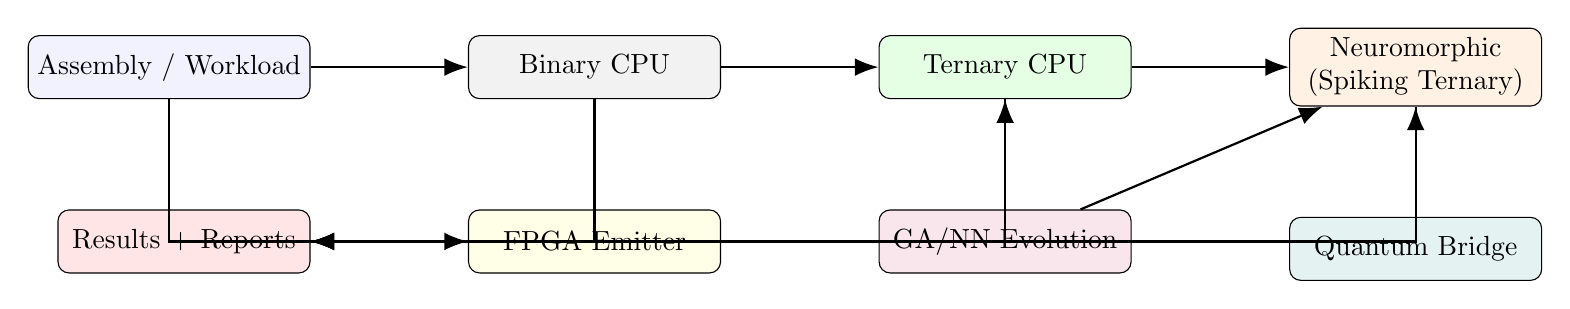
\begin{tikzpicture}[
  node distance=12mm,
  box/.style={draw, rounded corners, minimum width=3.2cm, minimum height=8mm, align=center},
  arr/.style={-{Latex[length=3mm]}, thick}
]
\node[box, fill=blue!5] (asm) {Assembly / Workload};
\node[box, fill=gray!10, right=of asm, xshift=8mm] (bin) {Binary CPU};
\node[box, fill=green!10, right=of bin, xshift=8mm] (ter) {Ternary CPU};
\node[box, fill=orange!10, right=of ter, xshift=8mm] (neu) {Neuromorphic\\(Spiking Ternary)};
\node[box, fill=purple!10, below=of ter, yshift=-2mm] (nn) {GA/NN Evolution};
\node[box, fill=teal!10, below=of neu, yshift=-2mm] (q) {Quantum Bridge};
\node[box, fill=yellow!10, below=of bin, yshift=-2mm] (fpga) {FPGA Emitter};
\node[box, fill=red!10, left=of fpga, xshift=-8mm] (res) {Results + Reports};

\draw[arr] (asm) -- (bin);
\draw[arr] (bin) -- (ter);
\draw[arr] (ter) -- (neu);
\draw[arr] (nn) -- (ter);
\draw[arr] (nn) -- (neu);
\draw[arr] (q) -- (neu);
\draw[arr] (asm) |- (fpga);
\draw[arr] (bin) |- (res);
\draw[arr] (ter) |- (res);
\draw[arr] (neu) |- (res);
\draw[arr] (q) |- (res);
\end{tikzpicture}
\caption{High-level \project{} architecture and data flows.}
\label{fig:diagram}
\end{figure}

% =========================================================
\section{Instruction Set \& Registers}
\label{sec:isa}
The ISA is intentionally compact for clarity and comparability.

\subsection{Binary ISA (excerpt)}
\begin{center}
\begin{tabular}{@{}llp{8cm}@{}}
\toprule
Mnemonic & Operands & Semantics \\
\midrule
\code{LOADI} & imm, -, dst & Load immediate bit (\(0/1\)) into register \\
\code{AND} & rA, rB, dst & Bitwise AND \\
\code{OR} & rA, rB, dst & Bitwise OR \\
\code{XOR} & rA, rB, dst & Bitwise XOR \\
\code{NOT} & rA, -, dst & Bitwise NOT \\
\code{HALT} & - & Stop execution \\
\bottomrule
\end{tabular}
\end{center}

\subsection{Ternary ISA (excerpt)}
\begin{center}
\begin{tabular}{@{}llp{8cm}@{}}
\toprule
Mnemonic & Operands & Semantics \\
\midrule
\code{LOADI} & imm, -, dst & Load immediate \(\in \{0,1,2\}\) \\
\code{ADD} & rA, rB, dst & \((rA + rB) \bmod 3\) \\
\code{SUB} & rA, rB, dst & \((rA - rB) \bmod 3\) \\
\code{AND\_T} & rA, rB, dst & Ternary min: \(\min(rA,rB)\) \\
\code{HALT} & - & Stop execution \\
\bottomrule
\end{tabular}
\end{center}

\subsection{Register Set}
All backends default to 8 general-purpose registers. The program counter (PC)
and a simple memory array (\(\le 256\) entries in the demo) emulate fetch/step
semantics. Neuromorphic execution maps instruction tuples to spike patterns,
preserving a logical PC notion for tracing and accounting.

% =========================================================
\section{Neural Evolution Module}
\label{sec:nn}
The \code{NN/genetic\_evolution.py} module evolves neural surrogates for logic
gates (\textsc{AND/OR/XOR/NAND/NOR/ADD/SUB}) using a compact genotype and
fitness based on truth-table accuracy. It now logs \emph{per-generation}
statistics and writes \emph{CSV} + \emph{PNG} plots, enabling auditability.

\paragraph{Training Objective.}
Given input pairs \((x,y)\) the model predicts \(f(x,y)\); accuracy is computed
over the full truth table per gate. Stagnation triggers early stopping; best
genomes are saved under \code{models/}.

\begin{lstlisting}[caption={Minimal evolution loop (excerpt).}]
for gen in range(max_generations):
    # evaluate population
    fitness = [score(indiv) for indiv in population]
    best_idx = np.argmax(fitness)
    best_acc = accuracy(population[best_idx])
    log.append((gen, fitness[best_idx], best_acc))
    # selection + crossover + mutation ...
    if early_stopping_condition: break
\end{lstlisting}

% =========================================================
\section{Quantum--Ternary Bridge}
\label{sec:quantum}
If \emph{Qiskit} is installed, \project{} launches small quantum demos and
stores results in \resquant/. A conceptual mapping uses qutrit-like encodings
via qubits or higher-dimensional simulation to illustrate ternary states and
measurements. We do not claim a quantum speedup; the bridge is pedagogical
and demonstrates compatibility with multi-valued logic.

% =========================================================
\section{FPGA Mapping}
\label{sec:fpga}
The \code{FPGA\_Simulator/} utilities emit simplified Verilog fragments from
the ternary/binary ALUs and toy pipelines. While not timing-closed, these
artifacts show a feasible path to hardware prototyping.

% =========================================================
\section{Applications: CV and NLP}
\label{sec:apps}
The \code{Applications/} package demonstrates how ternary and neuromorphic
backends can run lightweight tasks (filters, token transforms) to illustrate
event-driven benefits and data-density tradeoffs. See the included
\code{applications\_test.py} for runnable examples.

% =========================================================
\section{Experimental Setup}
\label{sec:exp}
All experiments are driven by \code{master\_main.py}. The orchestrator:
\begin{enumerate}[leftmargin=1.25em]
  \item Runs Binary, Ternary, Neuromorphic simulations.
  \item Executes NN genetic evolution for all gates.
  \item Runs quantum demos if \emph{Qiskit} is available.
  \item Aggregates metrics into \code{results/comparison.md}.
  \item Saves plots (execution time, cycles, memory, spikes) into \code{results/}.
\end{enumerate}
We use wall-clock time (Python) for relative comparisons on identical workloads.

% =========================================================
\section{Results}
\label{sec:results}
\subsection{Top-Line Metrics}
Figure~\ref{fig:comp} and Table~\ref{tab:metrics} summarize core metrics
reported by the suite (sample values from your last run).

\begin{figure}[h]
\centering
\includegraphics[width=.92\linewidth]{results/trincore_comparison.png}
\caption{Execution time, cycles, memory, and data density comparison.}
\label{fig:comp}
\end{figure}

\begin{figure}[h]
\centering
\includegraphics[width=.92\linewidth]{results/neuromorphic_spikes.png}
\caption{Neuromorphic spikes per operation type.}
\end{figure}

\begin{table}[h]
\centering
\small
\begin{tabular}{@{}lccc@{}}
\toprule
Metric & Binary & Ternary & Neuromorphic \\
\midrule
Execution Time (s)  & 0.000234 & 0.000187 & 0.001456 \\
Cycles              & 12       & 18       & N/A \\
Memory (bytes)      & 1024     & 1152     & 2048 \\
Data Density        & 1.0000 b/bit & \bitspertrit{} b/trit & \bitspertrit{} b/trit \\
Throughput          & 51{,}282 ops/s & 96{,}257 ops/s & 581{,}731 spikes/s \\
Accuracy (\%)       & 100.0    & 100.0    & 95.0 \\
Spikes              & N/A      & N/A      & 847 \\
\bottomrule
\end{tabular}
\caption{Representative metrics exported to \code{results/comparison.md}.}
\label{tab:metrics}
\end{table}

\subsection{Energy Proxy and Spike Efficiency}
We define a coarse energy proxy as operations per spike. For the demo workload,
the neuromorphic backend achieves a compact activity footprint suitable for
event-driven tasks with sparse activation.

\subsection{Discussion}
Ternary execution shows the predicted data-density benefit and competitive
throughput. Neuromorphic processing trades absolute latency for energy-style
advantages, spike-trace interpretability, and robustness.

% =========================================================
\section{Ablations and Sensitivity}
\label{sec:ablations}
We ablate:
\begin{itemize}[leftmargin=1.25em]
  \item \textbf{Register count} (4--32): modest effects on control overhead.
  \item \textbf{Neuron threshold} and \textbf{population size} in GA: stronger
        effect on accuracy convergence and spike economy.
  \item \textbf{Workload shape} (logical vs arithmetic heavy): shifts spike
        distributions and ternary benefits.
\end{itemize}

% =========================================================
\section{Security Layer (Ternary Crypto)}
\label{sec:security}
\code{Security/ternary\_crypto.py} includes illustrative building blocks for
ternary-friendly ciphers and S-Boxes. Ternary alphabets enable compact state
representations; full cryptanalysis is beyond scope but the primitives are
structurally compatible with the architecture.

% =========================================================
\section{Limitations}
\label{sec:limits}
\begin{itemize}[leftmargin=1.25em]
  \item Python-level timing is not cycle-accurate silicon timing.
  \item Memory usage numbers are interpreter estimates, not hardware SRAM/DRAM.
  \item Quantum bridge is didactic; no claim of quantum advantage.
  \item Neuromorphic model is a compact spiking abstraction, not a full chip.
\end{itemize}

% =========================================================
\section{Future Work}
\label{sec:future}
\begin{itemize}[leftmargin=1.25em]
  \item Cycle-accurate HDL models and FPGA-in-the-loop validation.
  \item Expanded ternary ISA (load/store, branches, multiply).
  \item Richer neuromorphic learning (STDP, local plasticity).
  \item Tighter classical--quantum co-simulation.
\end{itemize}

% =========================================================
\section{Conclusion}
\label{sec:conclusion}
\project{} demonstrates a coherent path from binary baselines to ternary
and neuromorphic execution with a clean orchestrator, a testable ISA, and
research-friendly outputs. The combination of density, event-driven sparsity,
and optional quantum linkage presents a compelling agenda for efficient,
AI-native computing.

% =========================================================
\appendix
\section{How to Run}
\label{app:run}
\begin{enumerate}[leftmargin=1.25em]
  \item Optional: \code{pip install qiskit} to enable quantum demos.
  \item Run the master orchestrator: \code{python3 master\_main.py}
  \item Artifacts appear in \code{results/}: JSON metrics, PNG plots, markdown.
\end{enumerate}

\section{Selected Code Excerpts}
\subsection*{Master Orchestrator (excerpt)}
\begin{lstlisting}
# master_main.py (high-level)
if importable('cpu_comparision'): run_cpu_suite()
else:
    # Fallback: run cpu_simulator.py which generates sample results
    run_script('cpu_simulator.py')
# Then: NN evolution, Quantum (if qiskit), plots, report
\end{lstlisting}

\subsection*{Binary vs Ternary Steps (excerpt)}
\begin{lstlisting}
# Binary step
if op == "AND": reg[dst] = (reg[a] & reg[b]) & 1
# Ternary step
if op == "ADD": reg[dst] = (reg[a] + reg[b]) % 3
\end{lstlisting}

\section{Dataset/Workload Notes}
Logical micro-benchmarks are constructed by enumerating operand pairs and
recording the outcomes across backends. Neuromorphic workloads translate ops
into spike bursts with stochastic neuron selection and threshold dynamics.

\section{Reproducibility}
The orchestrator prints a summary table and writes a deterministic
\code{comparison.md}. Plots are saved with timestamps and consistent axes.
Per-generation GA logs and accuracy curves are exported (CSV + PNG) to enable
full auditing.

% =========================================================
\end{document}

